{\bf Problem sheets from Oxford prelims Dynamics course: \url{https://courses.maths.ox.ac.uk/node/43927}}

\section{Sheet 1}
A first look at forces and dynamics: gravity and projectiles, fluid drag.

\subsection{}
\begin{mdframed}
  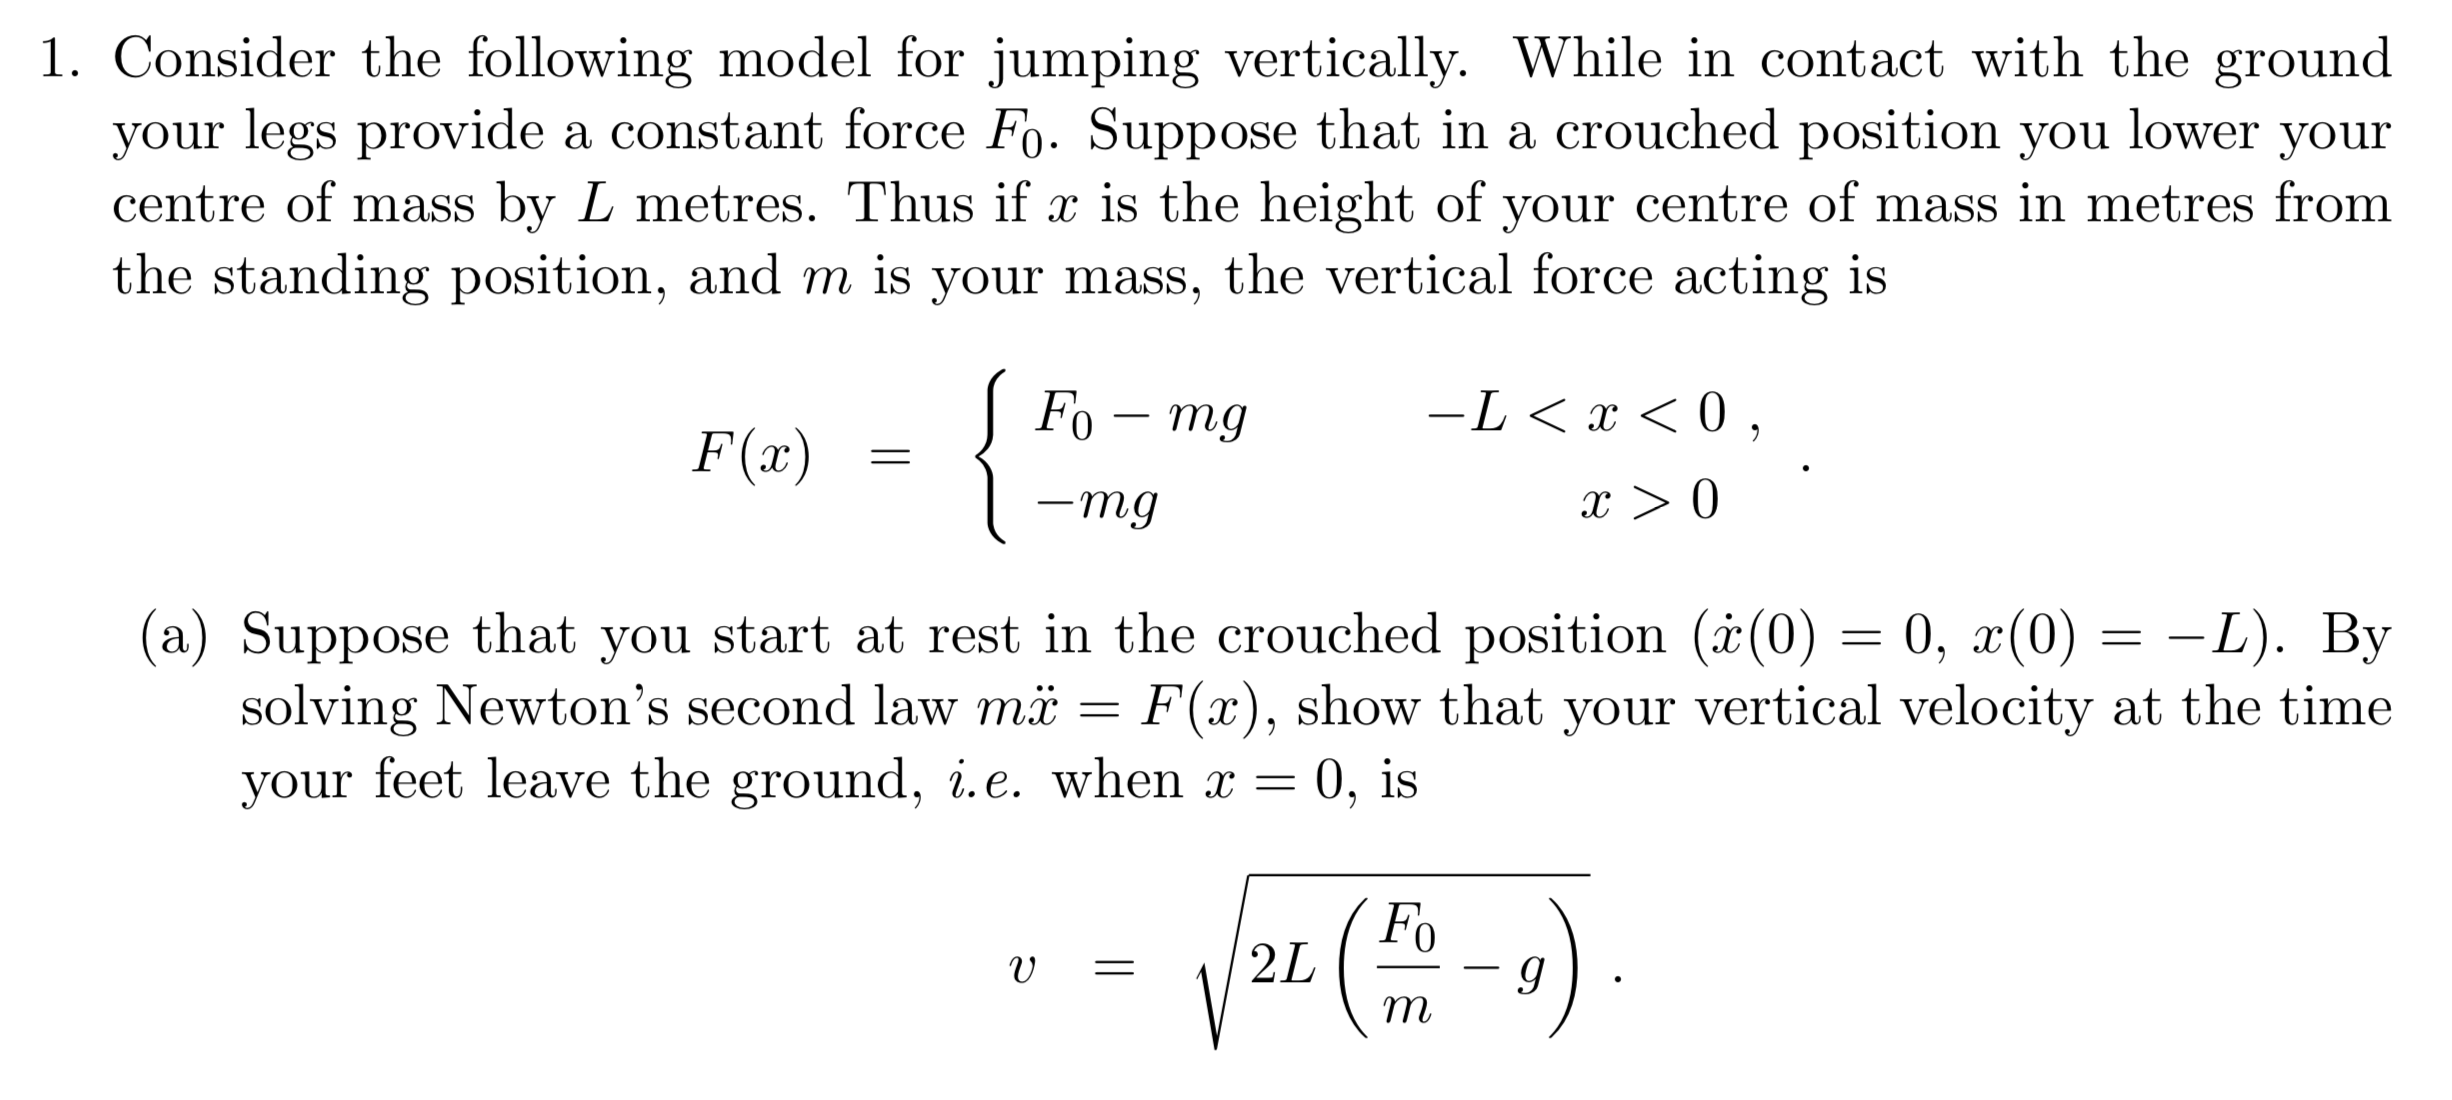
\includegraphics[width=400pt]{img/physics--classical-mechanics--oxford--dynamics-1-1.png}
\end{mdframed}

Strategy: we will solve the ODE for the trajectory $x(t)$, use this to find the time for which
$x(t) = 0$, and then find the velocity at that time.

The equation of motion while the legs are in contact with the ground is
$\ddot{x} = \dot{v} = \frac{F_0}{m} - g$. Thus from FTC
\begin{align*}
  v(t) - v(0) = v(t) = \dot{x} = \int_0^t \dot{v} \dt = \(\frac{F_0}{m} - g\)t.
\end{align*}
Applying FTC again gives the solution for the trajectory:
\begin{align*}
  x(t) - x(0) = x(t) + L = \int_0^t\dot{x} \dt = \frac{1}{2}\(\frac{F_0}{m} - g\)t^2.
\end{align*}

When $x = 0$ we have
\begin{align*}
  \frac{1}{2}\(\frac{F_0}{m} - g\)t^2 &= L \\
  t = \sqrt{\frac{2L}{\frac{F_0}{m} - g}},
\end{align*}
and the velocity at this time is
\begin{align*}
  \(\frac{F_0}{m} - g\)\sqrt{\frac{2L}{\frac{F_0}{m} - g}} &= \sqrt{2L\(\frac{F_0}{m} - g\)}.
\end{align*}


\begin{mdframed}
  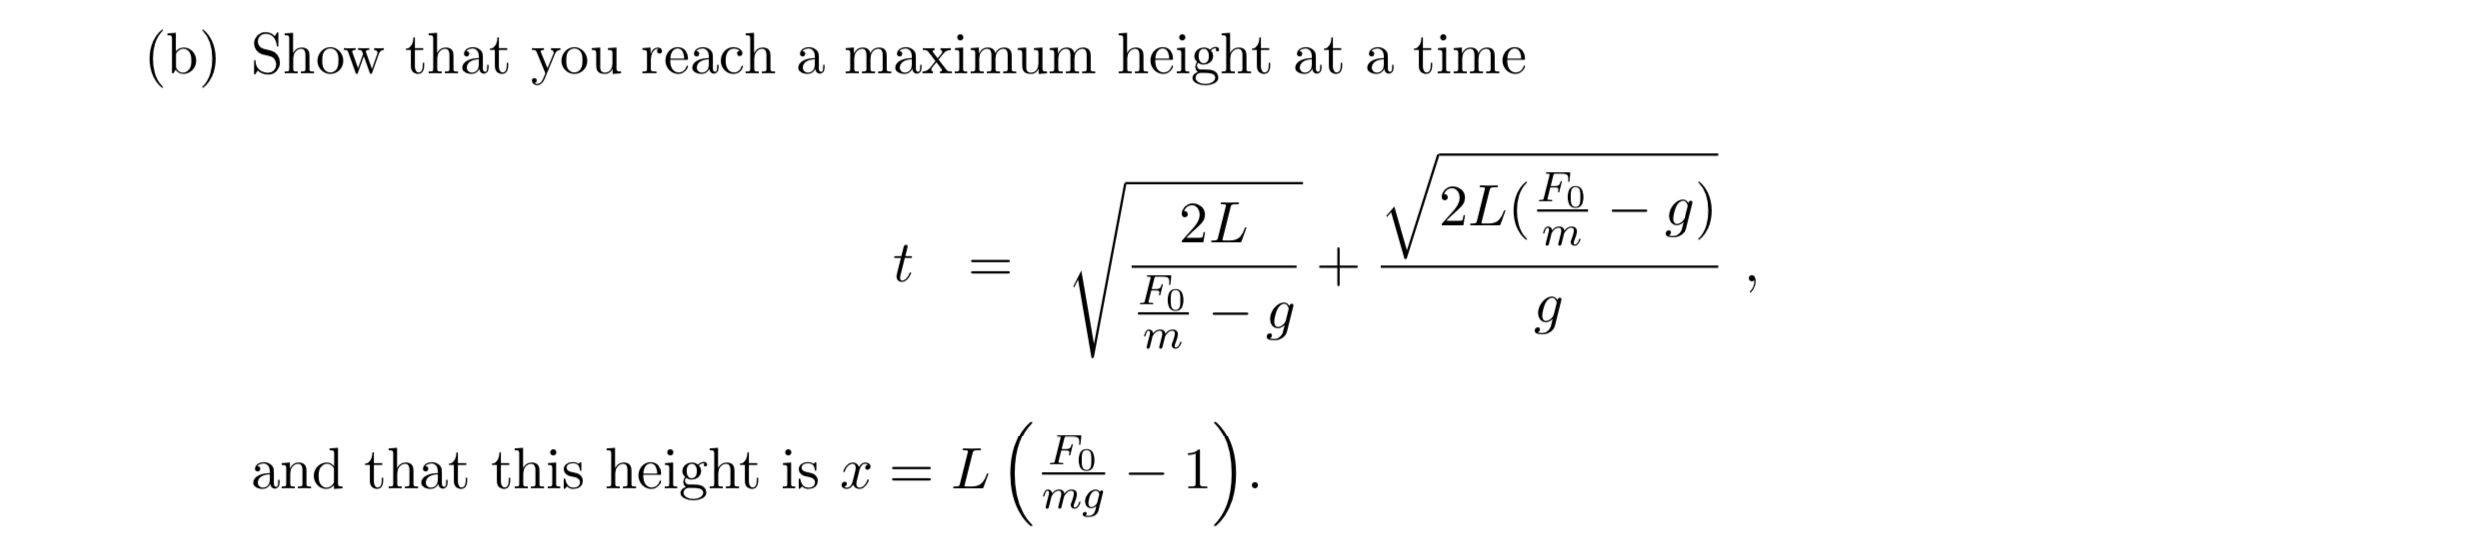
\includegraphics[width=400pt]{img/physics--classical-mechanics--oxford--dynamics-1-1-b.png}
\end{mdframed}

\section{Sheet 2}

\section{Sheet 3: Energy and equilibria}
\subsection{}
\begin{mdframed}
  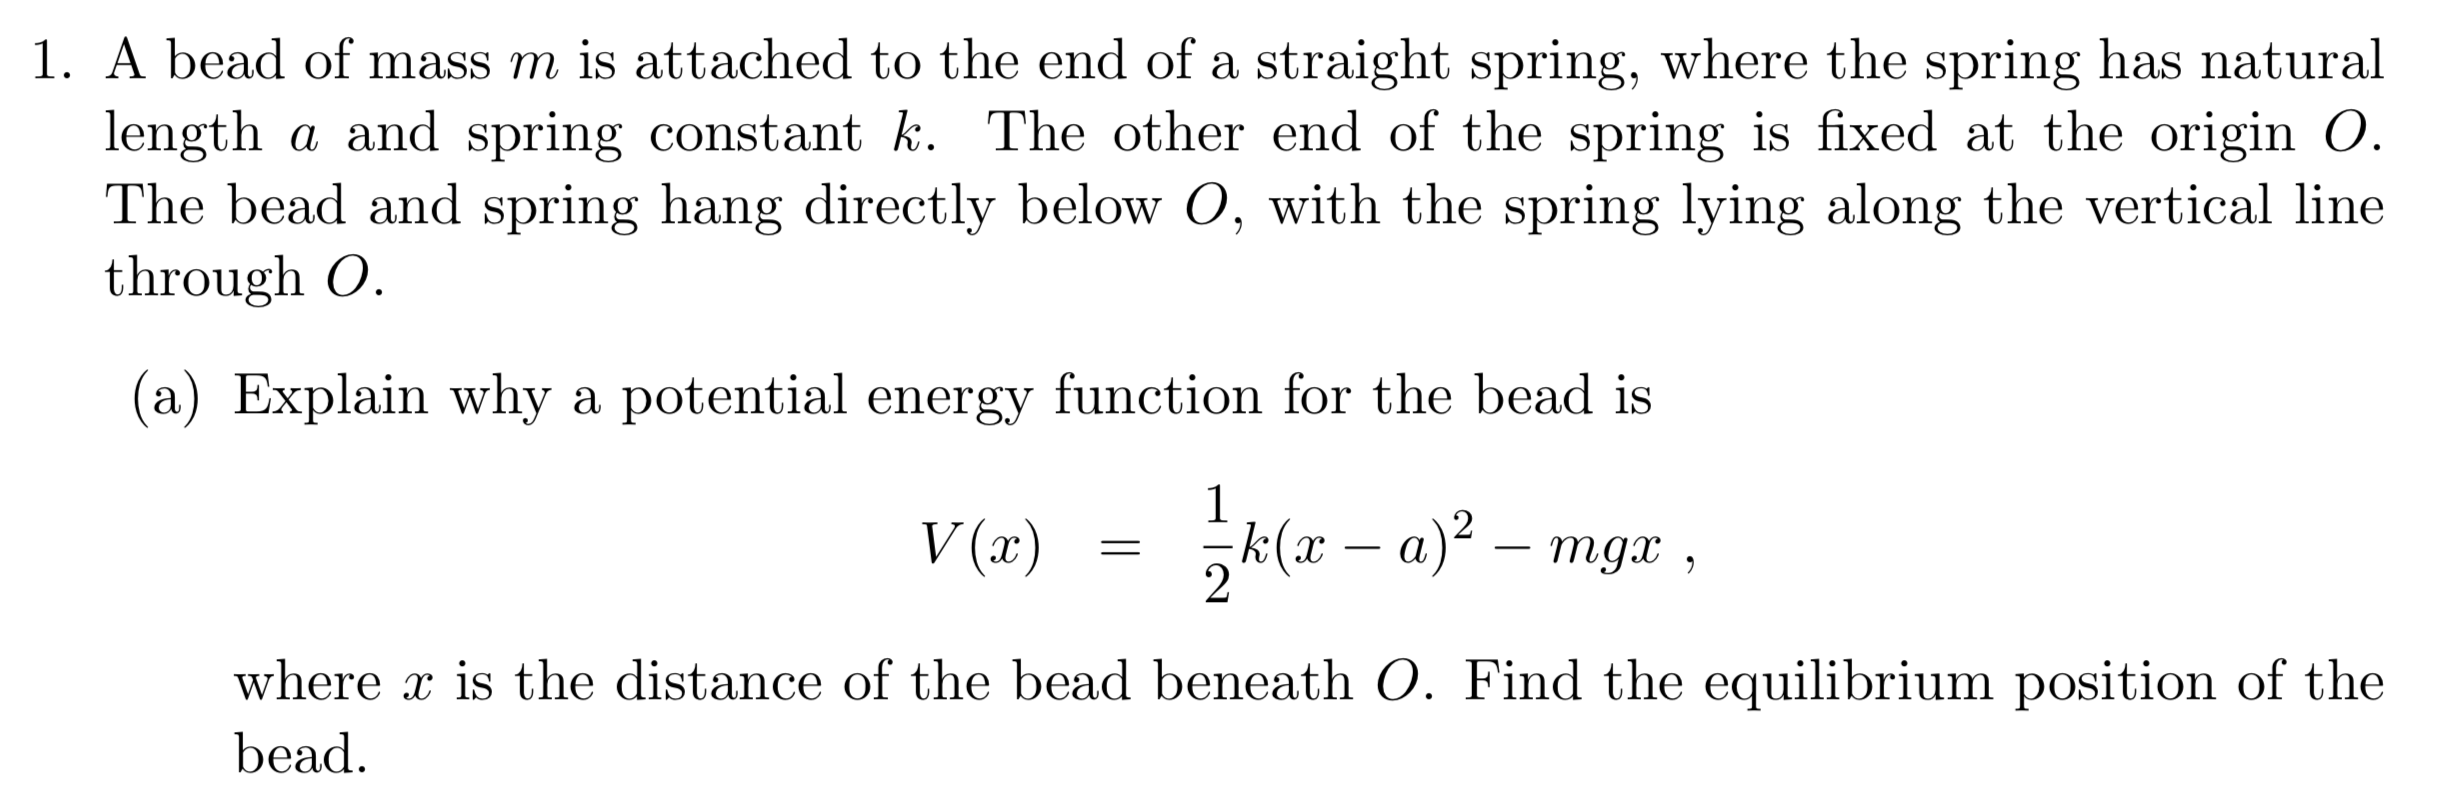
\includegraphics[width=400pt]{img/physics--classical-mechanics--oxford--dynamics-3-1.png}
\end{mdframed}
By definition, a potential energy function is
\begin{align*}
  V(x) = -\int_{x_0}^{x}F(x)\dx,
\end{align*}
where $x_0$ is arbitrary.

Let $x_0 = a$ (note that $x$ increases downwards). The force acting on the bead is then
$F(x) = -k(x - a) + mg$ and we have
\begin{align*}
  V(x)
  &= -\int_{x_0}^{x} \(-k(x - a) + mg\) \dx \\
  &= \Bigg[\frac{1}{2}k(x - a)^2 - mgx\Bigg]_a^x \\
  &= \frac{1}{2}k(x - a)^2 - mgx + mga.
\end{align*}
But $mga$ is constant, and potential energy is defined up to an arbitrary additive constant, so we
can choose
\begin{align*}
  V(x) &= \frac{1}{2}k(x - a)^2 - mgx.
\end{align*}

The bead's total energy is constant:
\begin{align*}
  E = V(x) + T(x).
\end{align*}

The equation of motion is
\begin{align*}
  \ddot{x} = -\frac{k}{m}(x - a) + g,
\end{align*}
hence
\begin{align*}
  \dot{x} =
\end{align*}

({\bf Strategy}: Solve to obtain $\dot{x}(t)$ and $x(t)$, then use these to find when $\dot{x}=0$?
How else can we know kinetic energy which requires knowing $\dot{x}$?)

At equilibrium, the bead's kinetic energy will be zero.